\documentclass[../thesis.tex]{subfiles}
% Separate preamble for this subfile. This preamble is loaded last, so one can override various functions before \begin{document}

% Better comment extension for Vscode colors these comments differently
% Normal comment color
% * Important information
% ! ALERT
% ? Question
% TODO stuff to do
% // This is strikethrough


\begin{document}

Before tackling spectral sets in higher dimensions, we first emphasize the importance of \cref{eq:zero_set_equation} and generalize it to higher dimensions. This result is similar to the general case in \cref{sec:indicator_zero_set}, although the distinction here is that we show it specifically in the case where $\Omega$ is the unit cube.
\begin{lemma}\label{lem:zero_set_jp_1_5}
    Let $\Omega = I^d$. The zero-set for $F_{\Omega}$ from \cref{eq:f_omega} %, in this case the function 
    %\begin{equation*}
    %    F_{I^d} (z):= \int_{I^d} e^{-2 \pi i \braa{z,t}} dt,
    %\end{equation*}
    is the set
    \begin{equation*}
        \Zstroke_{I^d} = \braqMed{ z = \brac{z_1,\dots,z_d}\in \R^d \setminus \braqMed{0} : \exists \space j \in \braqMed{1,\dots, d} \text{ such that } z_j \in  \intnozero}.
    \end{equation*}
\end{lemma}

\begin{proof} %! [Proof of  \cref{lem:zero_set_jp_1_5}] % Hvis proof med navn
    Given a vector $z \in \R^d$ we can factor $F_{\Omega}$ for $\Omega = I^d$ as follows
    \begin{align*}
        F_{I^d} (z) &= \int_{I^d} e^{-2 \pi i \braa{z,t}} dt\\
        &= \int_{I^d} e^{-2\pi i  (z_1 t_1 + \dots +z_d t_d)} dt\\
        &= \int_{I^d} e^{-2\pi i z_1 t_1}  \cdots e^{-2\pi i z_d t_d}  dt\\
        &= \int_{I} e^{-2\pi i z_1 t_1} \int_{I} e^{-2\pi i z_2 t_2}  \cdots \int_{I} e^{2\pi i z_d t_d}  dt_1 dt_2\dots dt_d\\ %! DENNE kan sløyfes
        &= \prod_{j=1}^d \int_I e^{-2\pi i z_j t_j} dt_j\\
        % &= \prod_{j=1}^d \frac{e^{2 \pi i z_j} -1}{2 \pi i z_j} % hvis JP F_\Omega
        &= \prod_{j=1}^d \frac{1-e^{-2 \pi i z_j}}{2 \pi i z_j} % hvis JP F_\Omega
    \end{align*}
    Note that if any $z_j = 0$, we interpret the corresponding factor in the product as $=1$. Furthermore, assume that $z\neq 0$ as this implies that at least one factor $z_j\neq 0$. In this case, observe that the equation is zero whenever at least one element $z_j\in \intnozero$. %using that the exponential equals one in this case. %* Forklaring, slettet
    Thus, the zero-set for $F_{I^d}$ is $\Zstroke_{I^d}$ which completes the proof. %* First sentence: In other words, reducing the total number of factors in the product.
    %If $z=0$, then we would have $e^{2\pi i z_j t_j} = 1$ and %* Trengs ikke, fordi vi er ute etter når det bir null
    %\begin{align*}
    %    F_{I^d} (0) = \prod_{j=1}^d \int_I 1 \space dt_j = \brac{\mes{I}}^d = 1.
    %\end{align*}
\end{proof}

Moreover, as an application of \cref{lem:zero_set_orthoganl_general} in combination with the specific zero-set for the unit cube $\Zstroke_{I^d}$ from \cref{lem:zero_set_jp_1_5}, we can formulate a result that closely resembles Keller's \namecref{thrm:keller_tiling} for tiling sets (\cref{thrm:keller_tiling}) \cite{lagariasOrthonormalBasesExponentials2000,jorgensenSpectralPairsCartesian2001}. The specific connection between the two results will become apparent later in \cref{chap:equivalence}.
\begin{lemma}[Spectral version of Keller's theorem]\label{lem:zero_set_AiSp}
    Let $\Lambda\subset \R^d$ be a discrete subset and $\Omega=I^d$. Then $\Lambda$ gives an orthogonal set of exponentials $E(\Lambda)$ if and only if
    \begin{equation*}%\label{eq:zero_set_inclusion}
        \Lambda - \Lambda \subseteq \Zstroke_{I^d} \cup \braq{0}.
    \end{equation*} 
\end{lemma}
%\begin{lemma}(Spectral version of Keller's theorem)  %* As it appears in Iosovich and Pedersen / Lagarias and Reeds. 
%    Let $\Lambda\subset \R^d$ be a discrete subset and $\Omega=I^d$. Then $\Lambda$ gives an orthogonal set of exponentials $E(\Lambda)$ if and only if given any two $\lambda,\lambda'\in \Lambda$ with $\lambda\neq\lambda'$, there exist a $j\in\braq{1,\dots,d}$ so that $\lambda_j- \lambda_j'\in \intnozero$.
%\end{lemma}

However, more useful, \cref{lem:zero_set_AiSp} also allows us to state the following result for spectral pairs. 
\begin{remark}\label{rem:zero_set_orthogonal}  %* One way implication, =>, which took a long time to find out. NOT the same as "Spectral Keller"
    If given a spectral pair $(I^d,\Lambda)$, it follows from \cref{def:spectral_set,lem:zero_set_AiSp} that the spectral pair property is equivalent to the set $E(\Lambda)$ is complete in $L^2(\Omega)$, and that
    \begin{equation*}  %\label{eq:zero_set_inclusion}
        \Lambda - \Lambda \subseteq \Zstroke_{I^d} \cup \braq{0}.
    \end{equation*}
\end{remark}

This \namecref{rem:zero_set_orthogonal} will be used later in \cref{thrm:class_all_shift_2d}.

%* ———————————————————————————————————————— Del 2, construction of spectra
In \cite{jorgensenSpectralPairsCartesian2001}, Jorgensen and Pedersen present a way of constructing spectral pairs in higher dimensions from spectral pairs in lower dimensions.

\begin{theorem}[Construction of spectra]\label{thrm:construction_spectra}
    Let $\brac{\Omega_1,\Lambda_1}$ be a spectral pair in $\R^{d_1}$, and let $\Omega_2$ be a set of positive finite measure in $\R^{d_2}$. Suppose for each $\lambda_1 \in \Lambda_1$ that $\lambfunc$ is a discrete subset of $\R^{d_2}$ such that $\brac{\Omega_2,\lambfunc}$ is a spectral pair. If 
    \begin{equation}\label{eq:construction_spectra}
        \Lambda = \braq{\brac{\lambda_1, \lambda_2}: \lambda_1\in \Lambda_1, \lambda_2 \in \lambfunc} 
    \end{equation}
    then $\brac{\Omega_1\times\Omega_2, \Lambda}$ is a spectral pair in $\R^{d_1+d_2}$ dimensions. 
\end{theorem}

\begin{remark}
    It can be helpful to think of $\lambfuncNoVar$ as a function that assigns a discrete subset in $\R^{d_2}$ to each $\lambda_1$-value such that $\brac{\Omega_2,\lambfunc}$ is itself a spectral pair. %* However, $\lambfunc$ should never be considered anything other than a set of points. 
\end{remark}

\begin{proof}[Proof of \cref{thrm:construction_spectra}]
    Given $\Lambda$ as  in \cref{eq:construction_spectra}, we start by showing that the set of exponentials $E(\Lambda)$ is orthogonal in $L^2\brac{\Omega_1 \times \Omega_2}$. For two elements $e_\lambda,e_{\lambda'} \in E(\Lambda)$ we have %the following inner product %Note that $t$ denotes the vector $(t_1,t_2)$ where $t_1 in \Omega_1$ and $t_2 \in \Omega_2$
    \begin{align*}
        \braa{e_\lambda,e_{\lambda'}}_{L^2\brac{\Omega_1 \times \Omega_2}} 
        &= \int_{\Omega_1} \int_{\Omega_2} e_{\lambda}(t) \overline{e_{\lambda'}(t)} dt_2 dt_1\\ 
        &= \int_{\Omega_1} \int_{\Omega_2} e^{2\pi i \braa{\lambda, t} } e^{-2\pi i  \braa{\lambda', t}} dt_2 dt_1\\ 
        &= \int_{\Omega_1} \int_{\Omega_2} e^{2\pi i \brac{\lambda_1 t_1+\lambda_2 t_2}} e^{-2\pi i\brac{\lambda_1' t_1+\lambda_2' t_2}} dt_2 dt_1\\ 
        &= \int_{\Omega_1} \int_{\Omega_2} e^{2\pi i \brac{\lambda_1- \lambda_1'}t_1} e^{2\pi i \brac{\lambda_2 - \lambda_2'}t_2} dt_2 dt_1\\ 
        &= \int_{\Omega_2} e^{2\pi i  \brac{\lambda_2- \lambda_2'}t_2} \bracMed{\int_{\Omega_1}  e^{2\pi i \brac{\lambda_1 - \lambda_1'}t_2} dt_1} dt_2.\\
        \intertext{Consider first $\lambda_1, \lambda_1' \in \Lambda_1$. If $\lambda_1 \neq \lambda_1'$, which results in $\lambda_2\in \lambfunc$ and $\lambda_2'\in \lambfuncGen{\lambda_1'}$, we would have that the inner integral will be zero because $\brac{\Omega_1, \Lambda_1}$ is a spectral pair. Conversely, if $\lambda_1 = \lambda_1'$ the resulting integral will factor as}
        &= \mes{\Omega_1} \int_{\Omega_2} e^{2\pi i  \brac{\lambda_2- \lambda_2'}t_2} dt_2.\\
        \intertext{Now, if one assumes $\lambda_2 \neq \lambda_2'$, then as both $\lambda_2, \lambda_2' \in \lambfunc$ the integral will be zero from the fact that $\brac{\Omega_2, \lambfunc}$ is a spectral pair. However, if $\lambda_2 = \lambda_2'$, observe that we have the case where $\lambda = \lambda'$, and}
        &= \mes{\Omega_1}\mes{\Omega_2} \neq 0.
    \end{align*}
    To show that $E(\Lambda)$ is complete in $L^2(\Omega_1 \times \Omega_2)$, let $f\in L^2\brac{\Omega_1 \times \Omega_2}$ and assume it is orthogonal to $\spn{E(\Lambda)}$. For all $e_\lambda \in E(\Lambda)$ the inner product is
    \begin{align*} %? REMEMBER t is a vector, i.e t=(t_1,t_2)
        \braa{e_\lambda,f}_{L^2\brac{\Omega_1 \times \Omega_2}}
        &= \int_{\Omega_1} \int_{\Omega_2} e_\lambda(t) \overline{f(t)} dt_1dt_2 \\
        &= \int_{\Omega_2} \int_{\Omega_1} e^{2\pi i  (\lambda_2 t_2+\lambda_1 t_1)} \overline{f(t_1,t_2)} dt_2 dt_1 \\
        &= \int_{\Omega_2} e^{2 \pi i \lambda_2 t_2} \int_{\Omega_1}e^{2 \pi i \lambda_1 t_1} \overline{f(t_1,t_2)} dt_1 dt_2
        %&= 0
    \end{align*}
    If we fix $\lambda_1$ and the integral vanishes for all $\lambda_2 \in \lambfunc$, then this implies 
    \begin{equation*}
        \int_{\Omega_1}e^{2 \pi i \lambda_1 t_1} \overline{f(t_1,t_2)} dt_1 = 0
    \end{equation*}
    for almost every $t_2\in \Omega_2$. This follows from $(\Omega_2,\lambfunc)$ being a spectral pair. Now, since $\lambda_1$ was arbitrary and $(\Omega_1,\Lambda_1)$ is a spectral pair we have that $f(t_1, t_2)=0$ for almost every $(t_1,t_2) \in \Omega_1 \times \Omega_2$. 
    This shows that $E(\Lambda)$ is complete in $L^2\brac{\Omega_1 \times \Omega_2}$, and concludes the proof that $(\Lambda, \Omega_1\times \Omega_2)$ is a spectral pair.
    %* Gammel variant var feil fordi rekkefølgen er klundrete når vi bruker L Funksjonen. Den er lettere å ta hensyn til som siste ting.
\end{proof}
%* ———————————————————————————————————————— Del 3, Eksempler på theoremet
Let us now give some examples using \cref{thrm:construction_spectra} to illustrate its ease of use and newfound flexibility \cite{jorgensenSpectralPairsCartesian2001}. 
\begin{example}\label{ex:first_construction}
    Let $\brac{\Omega_1,\Lambda_1}=\brac{I, \Z}$, which we know is a spectral pair in dimension $d_1=1$. Clearly $\brac{\Omega_2,\lambfunc}$ is also a spectral pair in dimension $d_2=1$ if $\Omega_2=I$ and $\lambfunc = \Z$ for all $\lambda_1 \in \Lambda_1$. Now, letting 
    %\begin{equation*}
    %    \lambfunc = \Z \text{ for all } \lambda_1 \in \Lambda_1
    %\end{equation*}
    %Now, letting 
    \begin{equation}\label{eq:first_construction}
        \Lambda  = \braqMed{\brac{\lambda_1,\lambda_2}: \lambda_1 \in \Z, \lambda_2 \in \lambfunc},
    \end{equation}
    it follows from \cref{thrm:construction_spectra} that $\brac{I^2, \Z^2}$ is a spectral pair in $1+1=2$ dimensions.
\end{example}

Recall our unproven \cref{lem:z_d_in_higer_d}. It is easy to see that applying \cref{thrm:construction_spectra} $d$ times will provide a proof of this result. \cref{ex:first_construction} is an example of a lattice spectrum, but the increase in dimension allows for more flexibility in that we can also construct spectra that are not lattices. %This becomes evident when looking at FIGUREXX, which illustrates the grid-like pattern of a lattice. 

%! FIGURE INPUT



\begin{figure}[t]%h!
    \centering
    \begin{subfigure}{.47\textwidth}
        \centering
        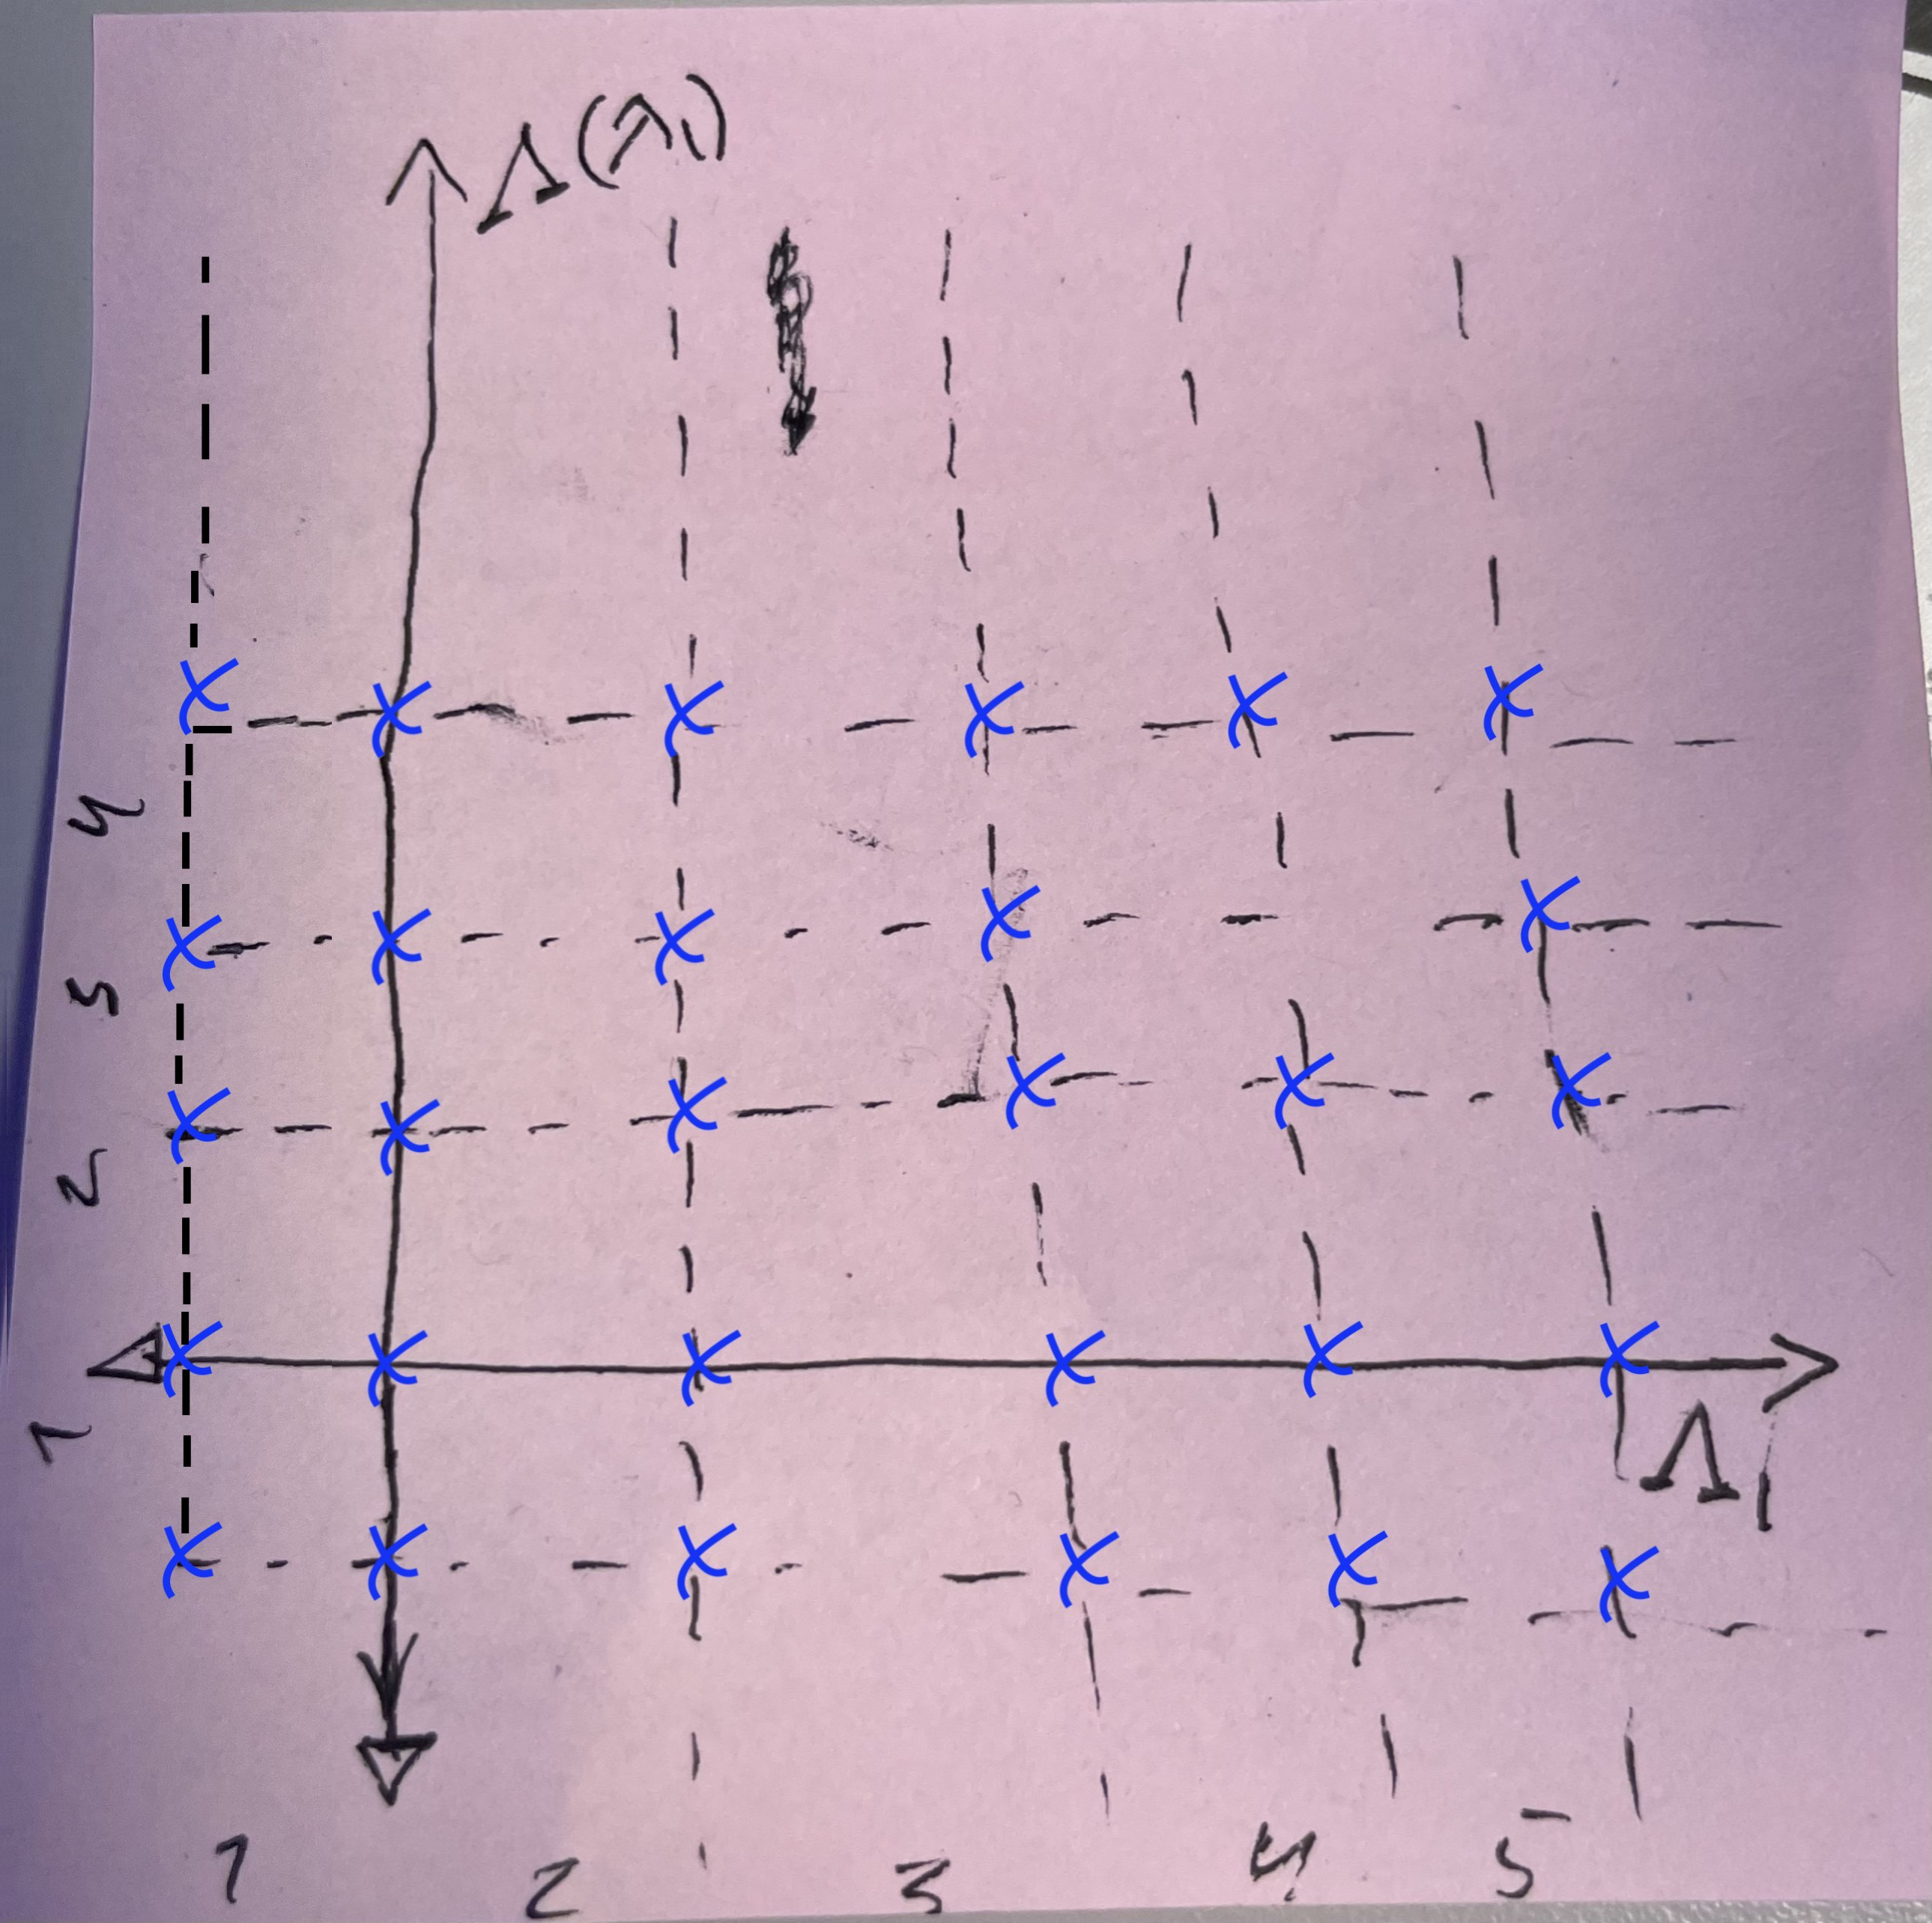
\includegraphics[width=0.9\linewidth]{spec_no_shift.jpg}
        \caption{Lattice spectra}
        \label{fig:lattice_spectra}
    \end{subfigure}\quad
    \begin{subfigure}{.47\textwidth}
        \centering
        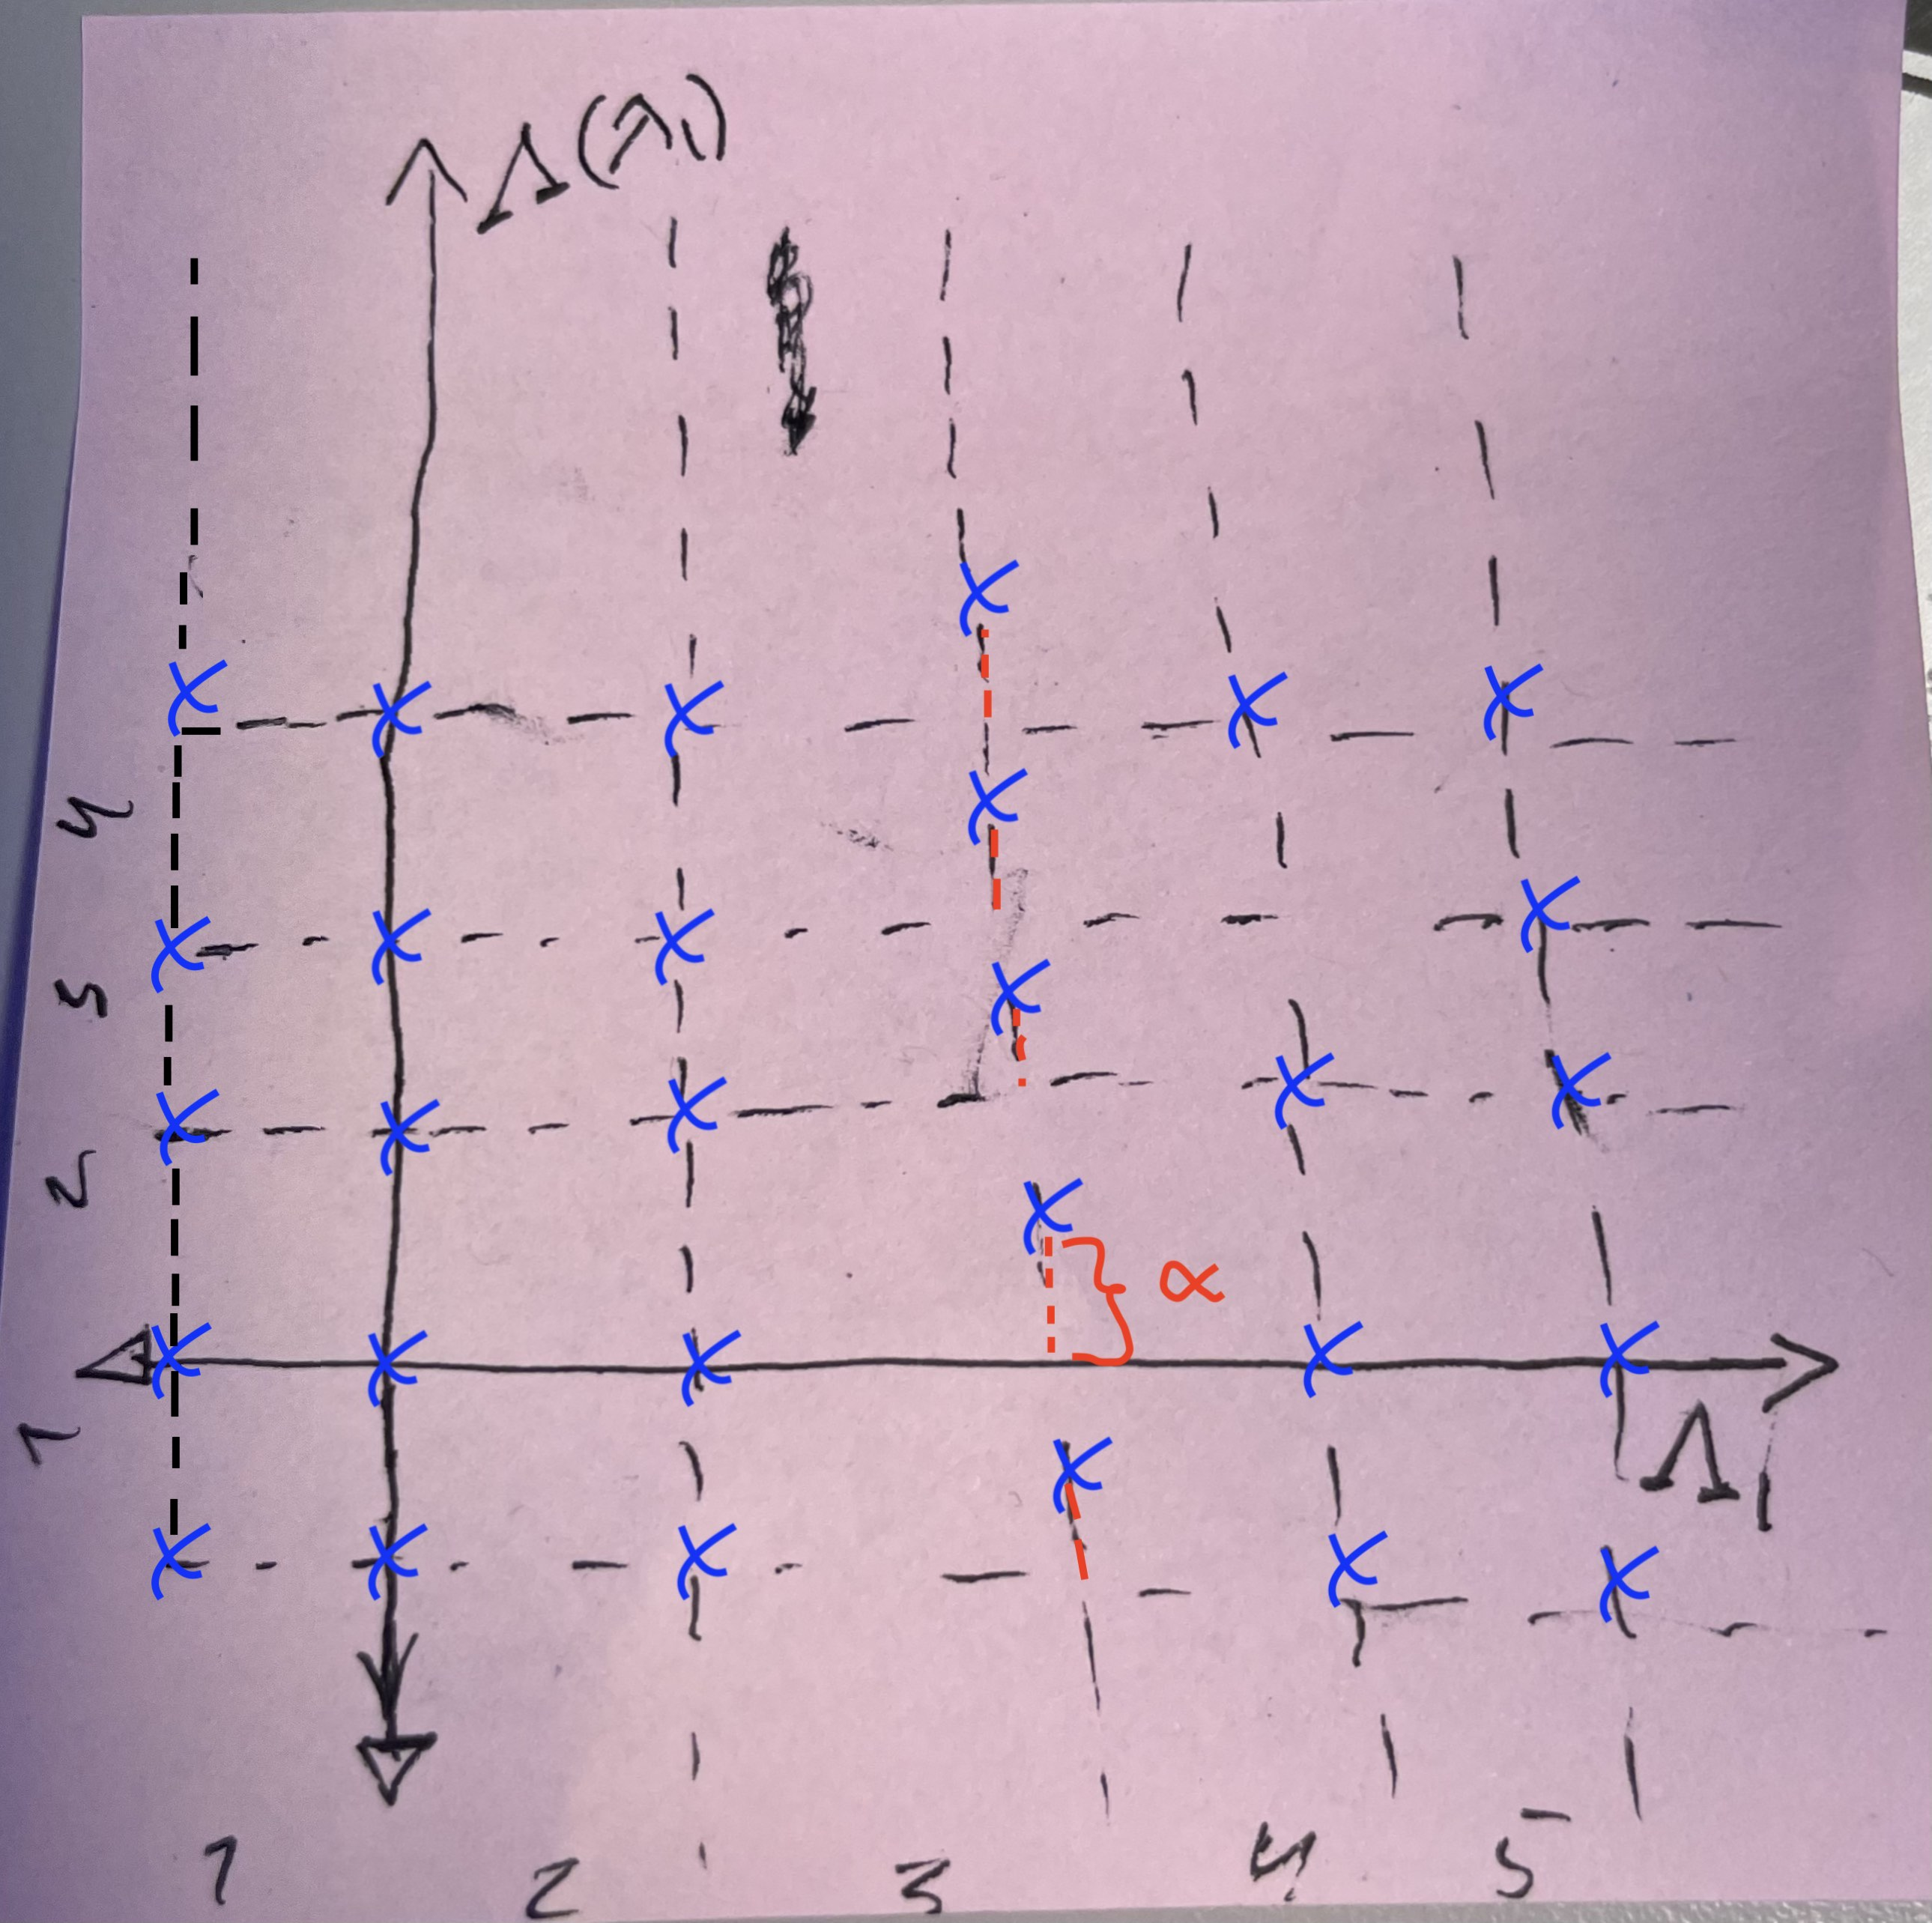
\includegraphics[width=0.9\linewidth]{spec_single_shift.jpg}
        \caption{Single shift vertical}
        \label{fig:single_shift_vertical}
    \end{subfigure}\\
    \begin{subfigure}{.47\textwidth}
        \centering
        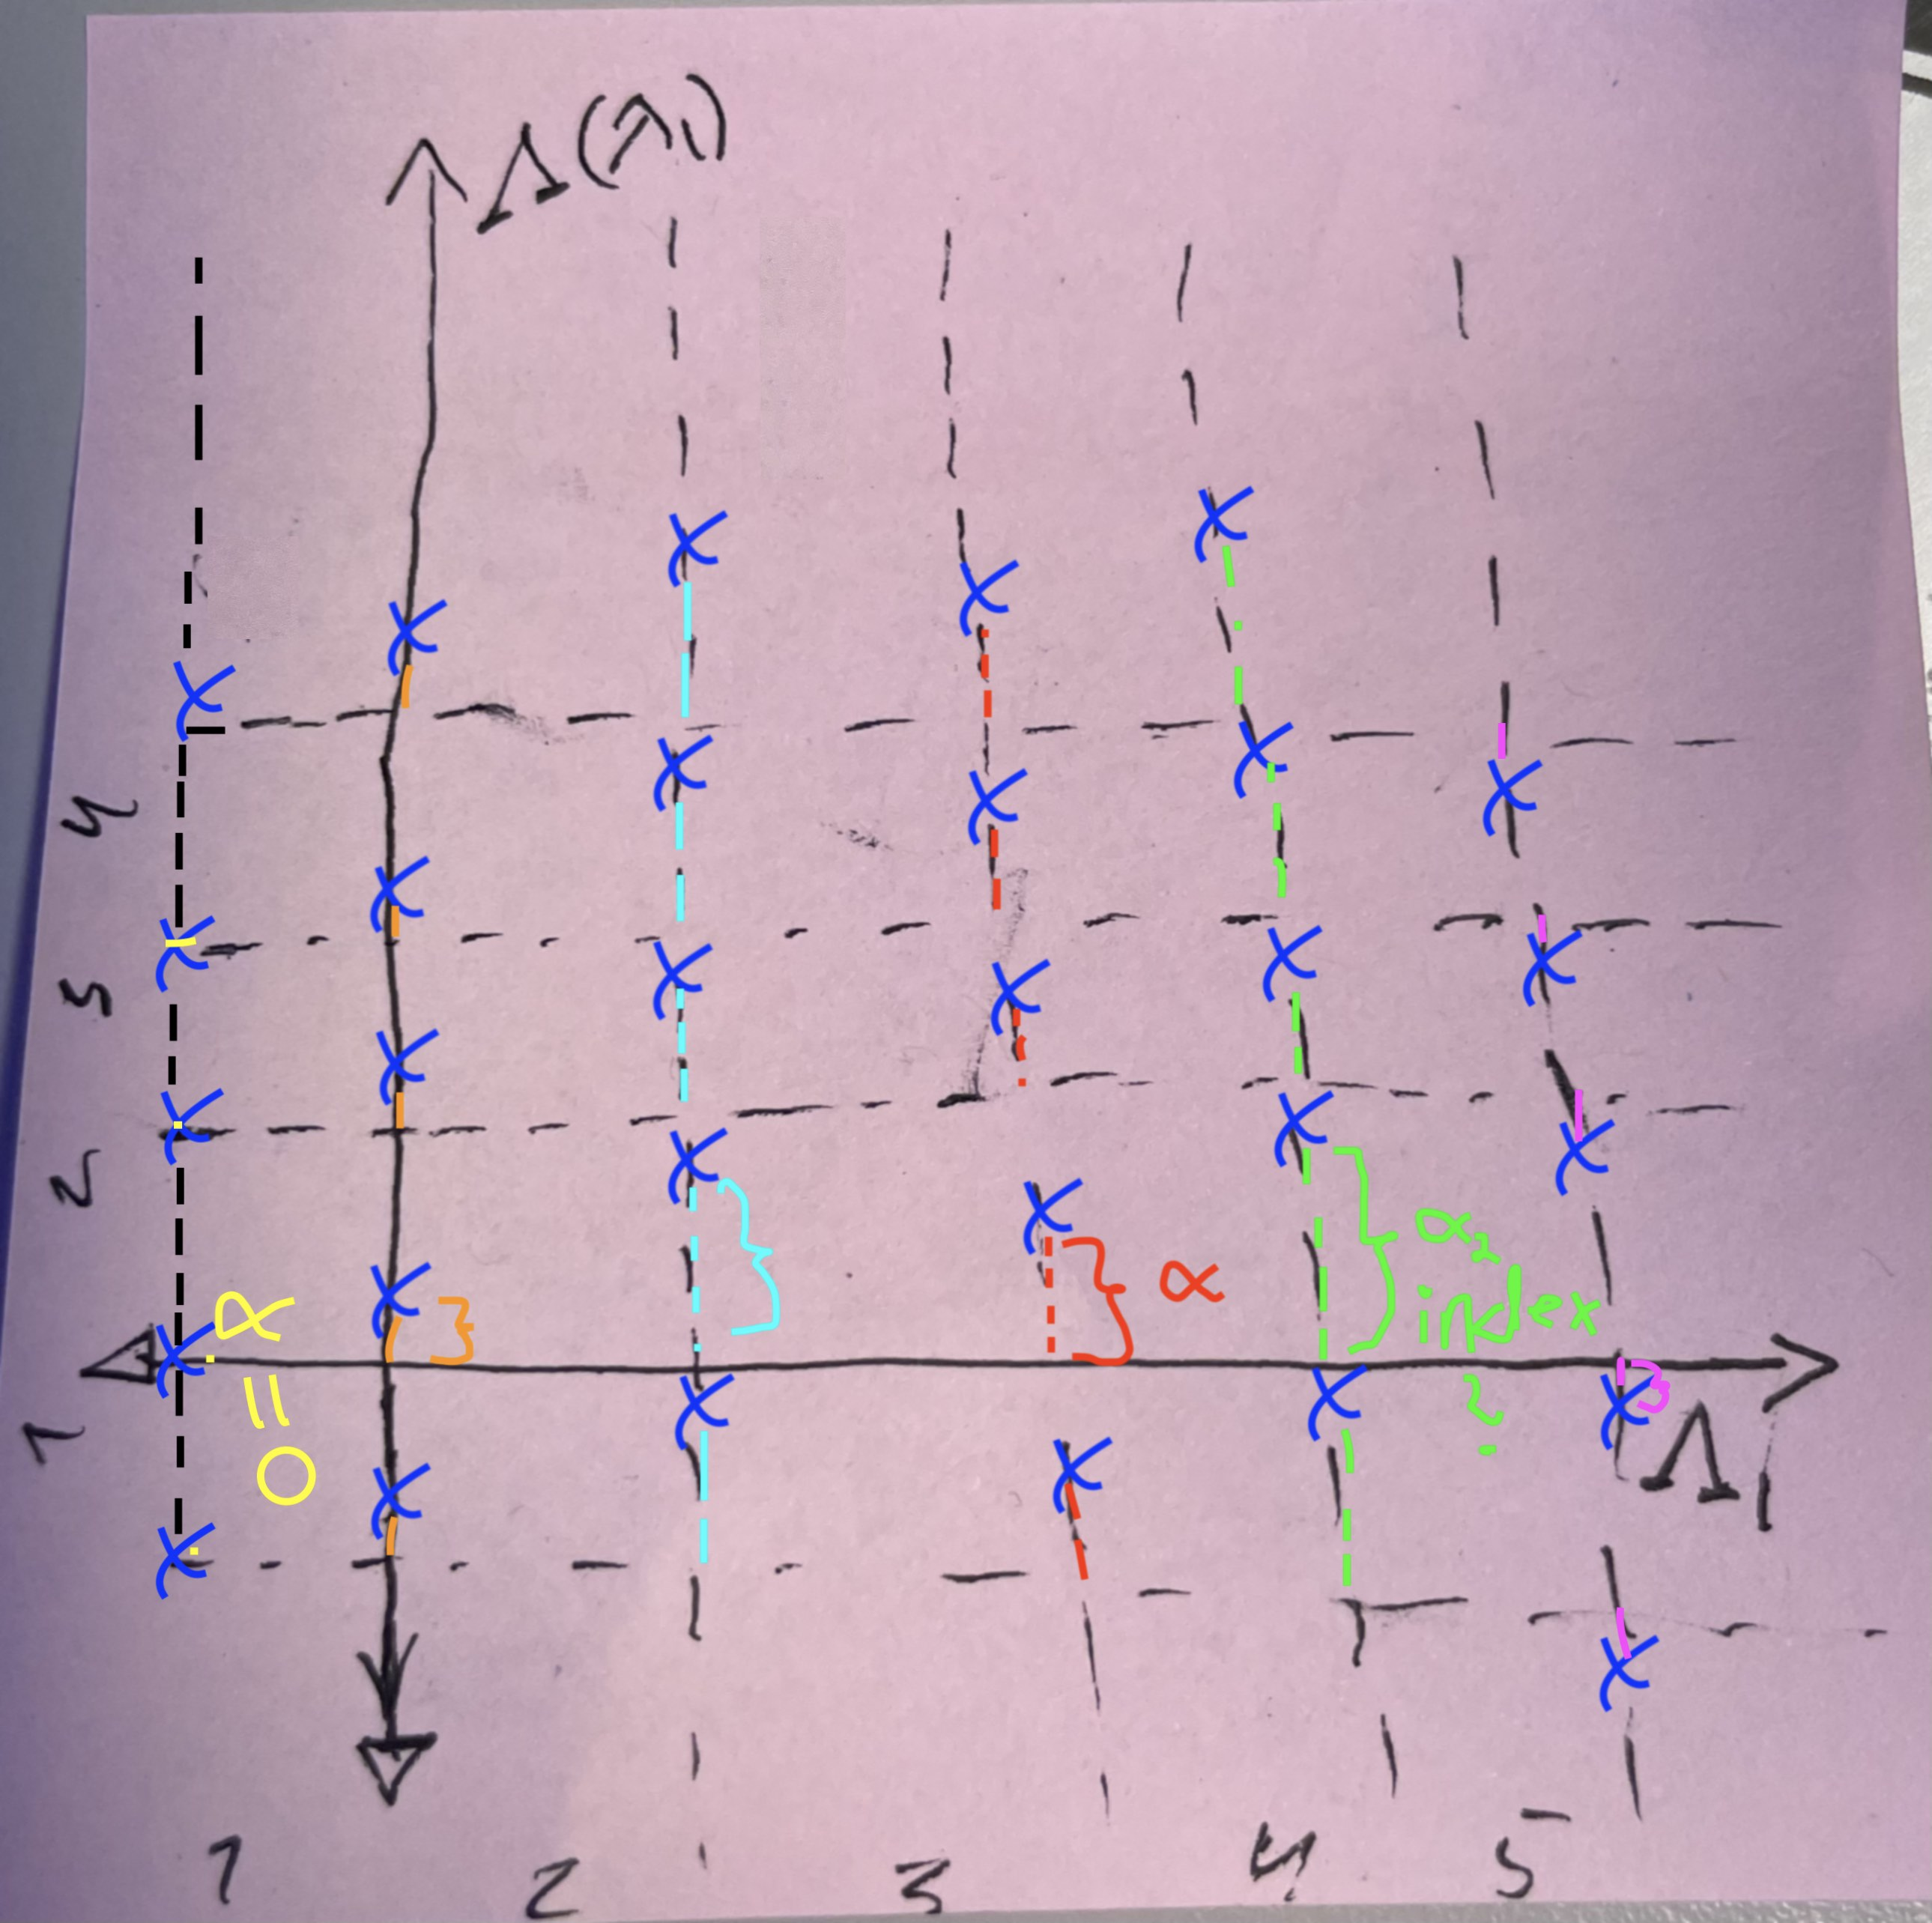
\includegraphics[width=0.9\linewidth]{multiple_shift_left_zero.jpg}
        \caption{Multiple individual shifts vertical}
        \label{fig:multiple_shift_vertical}
    \end{subfigure}\quad
    \begin{subfigure}{.47\textwidth}
        \centering
        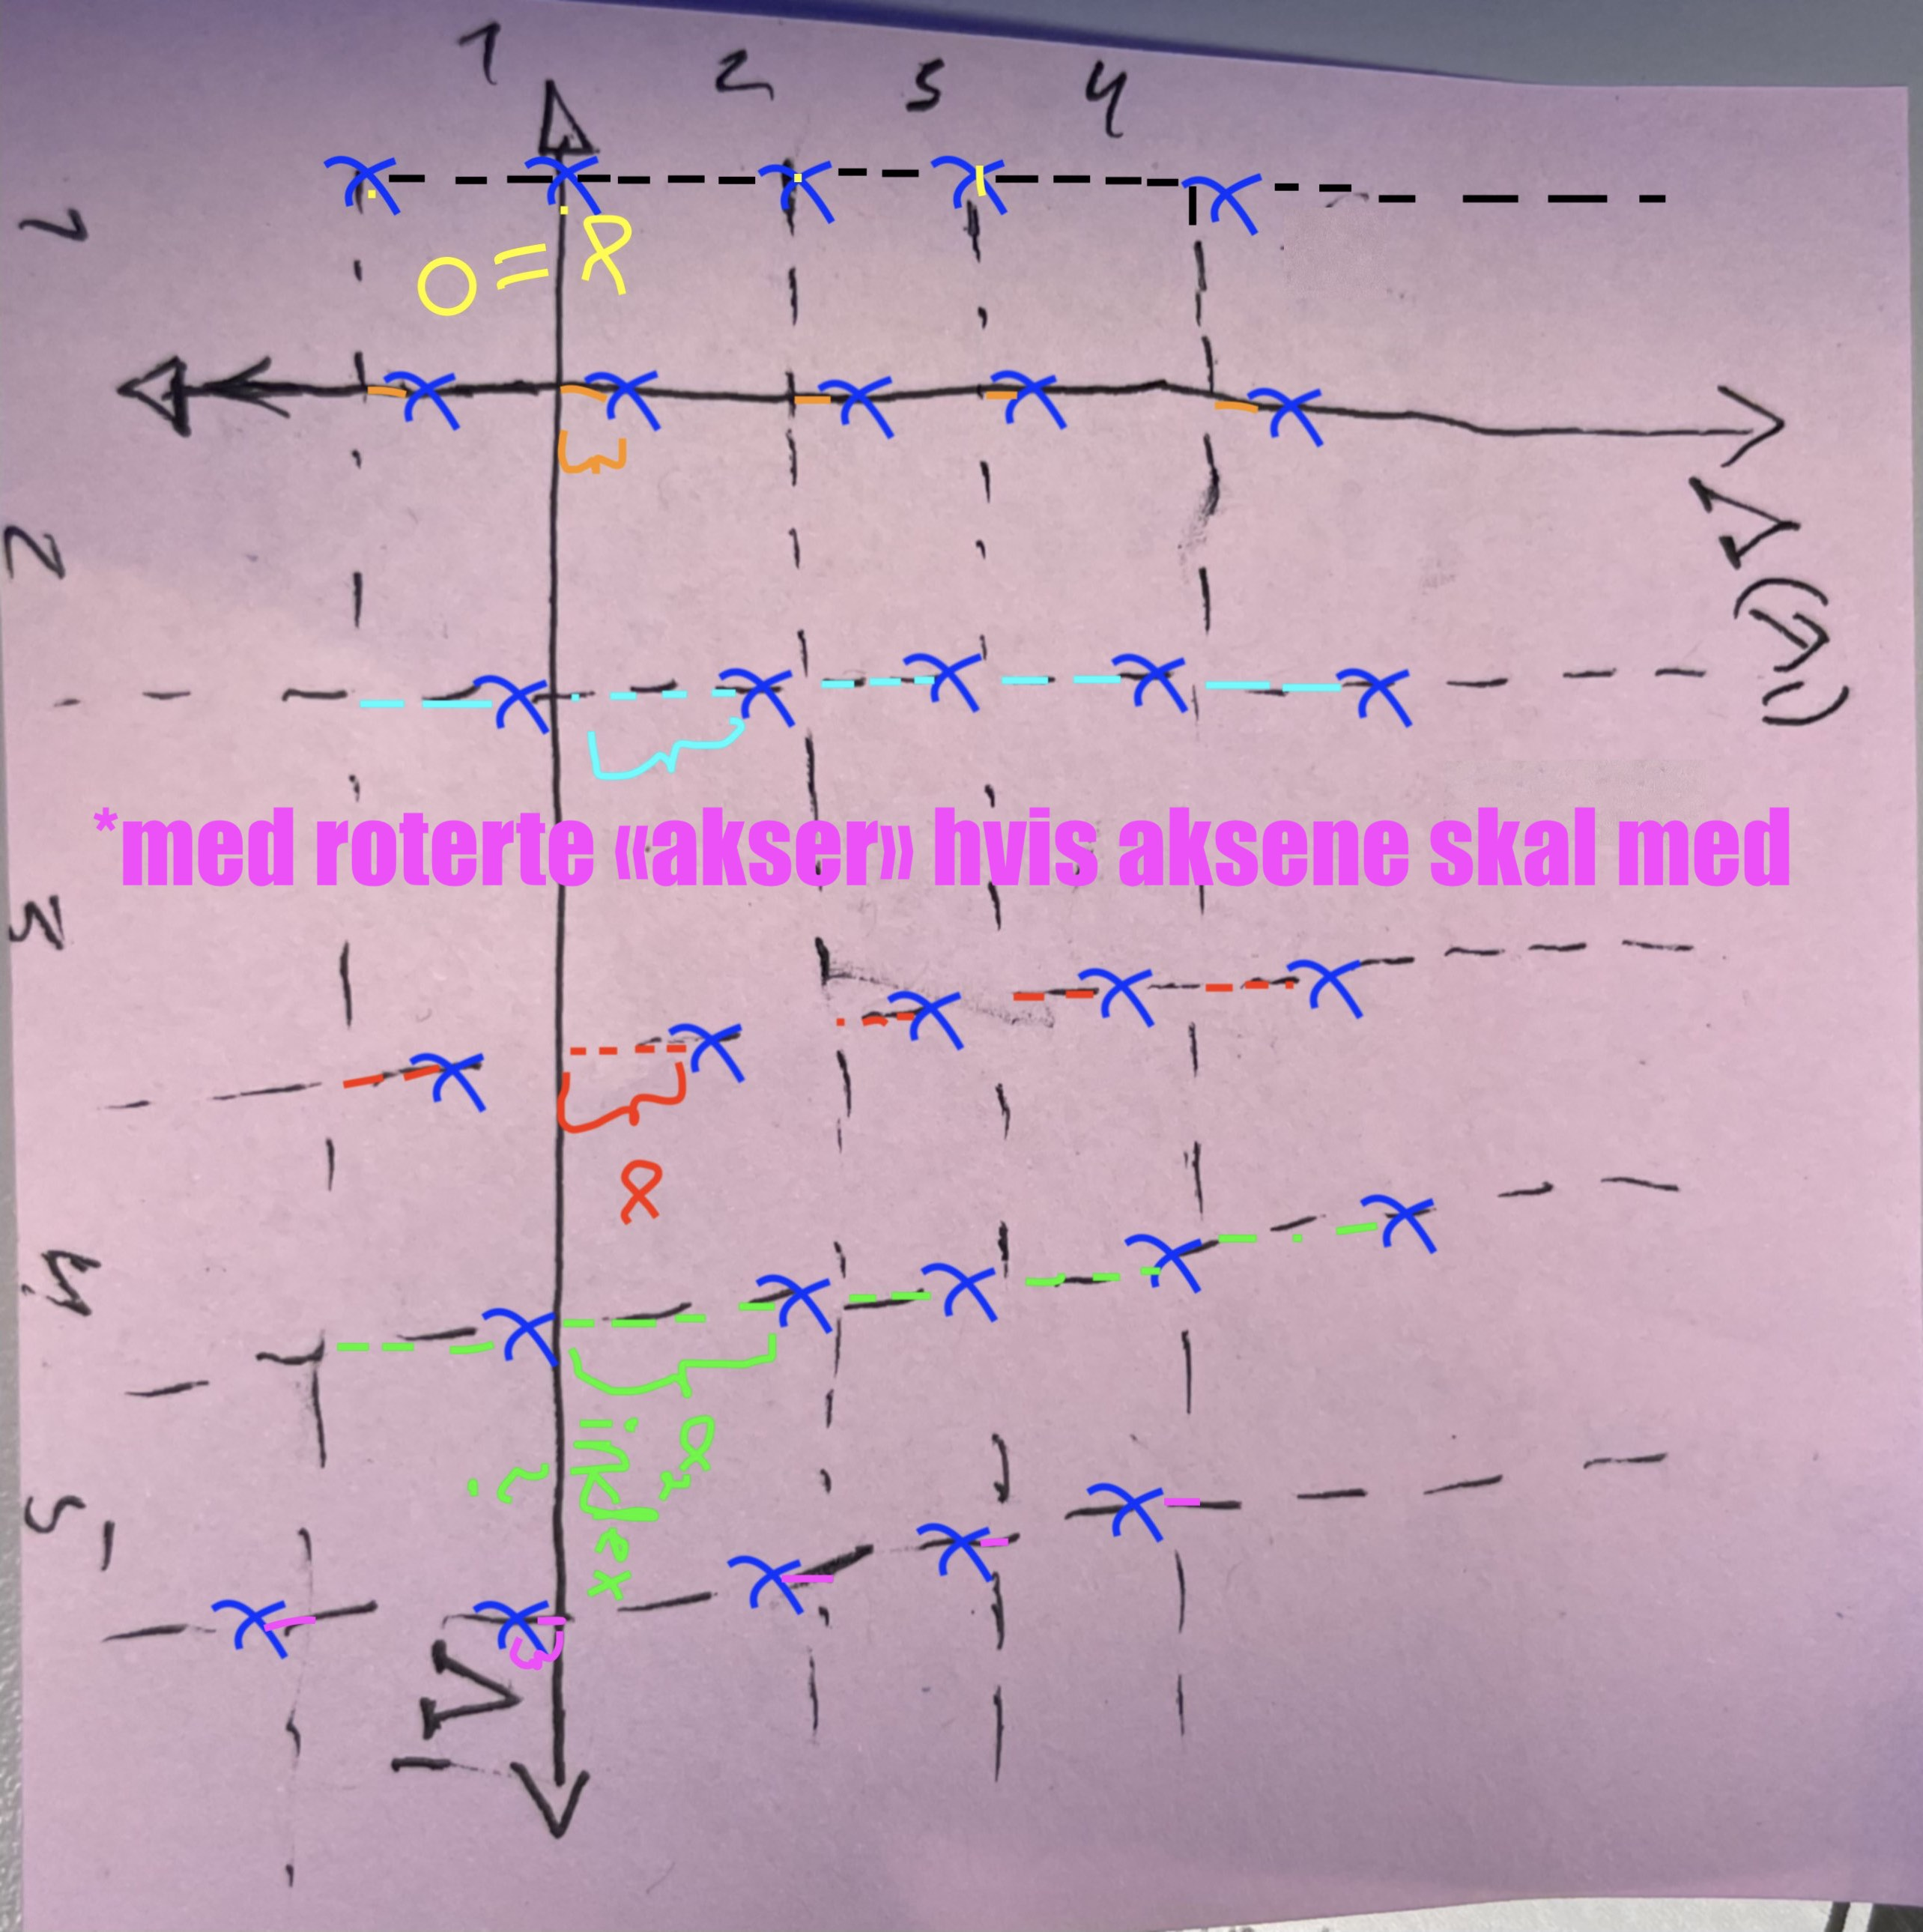
\includegraphics[width=0.9\linewidth]{multiple_shift_left_zero_horizontal.jpg}
        \caption{Multiple individual shifts horizontal}
        \label{fig:multiple_shift_horizontal}
    \end{subfigure}
    \caption{Illustration of the following pair of spectral pairs. In \labelcref{fig:lattice_spectra} we have $\brac{I,\Z}$ and $\brac{I,\lambfunc}$.  In \labelcref{fig:single_shift_vertical} we have $\brac{I,\Z}$ and $\brac{I,\lambfunc}$, where $\lambfunc$ is given by \labelcref{eq:single_shift_vertical}. In \labelcref{fig:multiple_shift_vertical} we have $\brac{I,\Z}$ and $\brac{I,\lambfunc}$, where $\lambfunc$ is given by \labelcref{eq:multiple_shit_func}. In \labelcref{fig:multiple_shift_horizontal} we have $\brac{I,\Z+0.4}$ and $\brac{I,\lambfunc}$, where $\lambfunc$ is given by \labelcref{eq:multiple_shit_func}.}
    \label{fig:spectra_figures}
\end{figure}


\begin{example}\label{ex:single_shift_vertical}
    Letting $\Omega_1=\Omega_2 = I$ in \cref{thrm:construction_spectra}, we can choose $\Lambda_1 = \Z$ and 
    \begin{align}\label{eq:single_shift_vertical}
        \lambfunc = \begin{cases}        
            \Z & \text{for all } \lambda_1 \in \Lambda_1\setminus\braq{\lambda_1'},\\        
            \Z+\beta & \text{if } \lambda_1=\lambda_1',\text{ where } \beta \in \mathbb{R}.   
        \end{cases}
    \end{align}
    Then the resulting spectrum for $I^2$ will be
    \begin{equation}\label{eq:lam_single_shift_vertical}
        \Lambda = \braqMed{\brac{\lambda_1, \lambda_2}: \lambda_1\in \Z, \lambda_2 \in \lambfunc},
    \end{equation}
    with $\lambfuncNoVar$ given by \labelcref{eq:single_shift_vertical}. This spectrum is illustrated in \cref{fig:single_shift_vertical} with $\beta = 0.5$.
\end{example} %* for the two spectral pairs $\brac{I,\Z}$ and $\brac{I,\lambfunc}$. NEI, dette er et valg av L(.) mer enn et spektrum.  og i den grad det er et spektrum så er jo hvert enkelt L(.) et spektrum for I.
%! Sigrid wants to delete "value" in the next sentence
Furthermore, there is no reason only to consider one shift for one $\lambda_1'$ as done in \cref{ex:single_shift_vertical}. 
\begin{example}\label{ex:multiple_shift_vertical}
    Again, letting $\Omega_1=\Omega_2 = I$ in \cref{thrm:construction_spectra}, we can choose $\Lambda_1 = \Z$ and 
    \begin{align}\label{eq:multiple_shift_vertical}
        \lambfunc = \begin{cases}
            & \text{ \space \space }\vdots\\        
            \Z+0 & \text{for } \lambda_1 = -1 \in \Lambda_1\\
            \Z+0.3 & \text{for } \lambda_1 = \text{\space\space\space} 0 \in \Lambda_1,\\
            \Z+0.7 & \text{for } \lambda_1 = \text{\space\space\space} 1 \in \Lambda_1,\\
            \Z+0.4 & \text{for } \lambda_1 = \text{\space\space\space} 2 \in \Lambda_1,\\
            \Z+0.6 & \text{for } \lambda_1 = \text{\space\space\space} 3 \in \Lambda_1,\\
            \Z-0.4 & \text{for } \lambda_1 = \text{\space\space\space} 4 \in \Lambda_1,\\
            & \text{ \space \space }\vdots
        \end{cases}
    \end{align}
    Then the resulting spectrum for $I^2$ will be
    \begin{equation}\label{eq:lam_multiple_shift_vertical}
        \Lambda = \braqMed{\brac{\lambda_1, \lambda_2}: \lambda_1\in \Z, \lambda_2 \in \lambfunc},
    \end{equation}
    with $\lambfuncNoVar$ given by \labelcref{eq:multiple_shift_vertical}. This spectrum is illustrated in \cref{fig:multiple_shift_vertical}. Note that there is no reason to consider shifts $\beta \geq 1$ as we can always write the shift as some value $n+\beta$ where $n\in \Z$ and $\beta \in [0,1)$.
\end{example}
%
\begin{remark}\label{rem:switch_lambda}
    In addition to choosing $\Omega_1=\Omega_2 = I$ and $\lambfuncNoVar$ given by \labelcref{eq:multiple_shift_vertical} as in \cref{ex:multiple_shift_vertical}, we can shift $\Lambda_1$ with, for example, $\alpha = -0.4$. %as illustrated in \cref{fig:multiple_shift_horizontal}.
    At last, we can also change the roles of $\Lambda_1$ and $\Lambda_2$. That is,
    \begin{equation}\label{eq:lam_multiple_shift_horizontal}
        \Lambda = \braqMed{\bracMed{\lambda_1, \lambda_2}: \lambda_1 \in \lambfuncGen{\lambda_2}, \lambda_2 \in \Lambda_2 },
        %\Lambda = \braqMed{\begin{pmatrix}\lambda_1 \\ \lambda_2 \end{pmatrix}: \lambda_1 \in \Z, \lambda_2 \in \lambfunc}
        %\Lambda = \begin{pmatrix}\lambfuncGen{\lambda_2} \\ \Lambda_2 \end{pmatrix}
    \end{equation}
    which is illustrated in \cref{fig:multiple_shift_horizontal}, is also a spectrum for $I^2$.
\end{remark}
As has been observed, increasing the dimension from one to two opens up several new possibilities in our choices for the spectrum. We summarize this flexibility seen in \cref{ex:first_construction,ex:single_shift_vertical,ex:multiple_shift_vertical} in the following \namecref{lem:beta_shift} \cite{jorgensenSpectralPairsCartesian2001}.
%* ———————————————————————————————————————— Del 4, Lemma som fanger den nye fleksibiliteten
\begin{lemma}\label{lem:beta_shift}
    Let $\brac{\Omega_1,\Lambda_1}$ and $\brac{\Omega_2,\Lambda_2}$ be spectral pairs in dimensions $d_1$ and $d_2$, respectively. Furthermore, define an arbitrary function $\betafunc: \Lambda_1 \rightarrow \R^{d_2}$, and let
    % $\betafunc: \Lambda_1 \rightarrow \R^{d_2}$ to denote the shift in the spectrum for $\Omega_2$ at each $\lambda_1$-value, and let %* unødvendig
    \begin{equation}
        \Lambda = \Lambda_\beta
        = \braqMed{\begin{pmatrix}
            \lambda_1 \\
            \lambda_2+\betafunc(\lambda_1)
            \end{pmatrix}
        : \lambda_1 \in \Lambda_1 \text{ and } \lambda_2 \in \Lambda_2}.
    \end{equation}
    Then $\brac{\Omega_1 \times \Omega_2,\Lambda_\beta}$ is a spectral pair in $d_1+d_2$ dimensions. 
\end{lemma}
%\begin{proof}  %! No proof is needed here
%    As we assumed that $\brac{\Omega_2,\Lambda_2}$ is a spectral pair, it follows directly from \cref{lem:spectrum_shift_is_spectrum} that $\brac{\Omega_2,\Lambda_2+\beta}$ is also a spectral pair for any $\beta \in \R^{d_2}$ (with elements populated by $\betafunc(\lambda_1)$)
%\end{proof}
\begin{remark}\label{rem:beta_shift}
    We can also shift the spectrum for $\Omega_1$ by a vector $\alpha \in \R^{d_1}$ to obtain the spectrum 
    \begin{equation*}
        \Lambda = \Lambda_{\alpha,\beta} 
        = \braqMed{\begin{pmatrix}
            \lambda_1 +\alpha\\
            \lambda_2+\betafunc(\lambda_1)
            \end{pmatrix}
        : \lambda_1 \in \Lambda_1 \text{ and } \lambda_2 \in \Lambda_2}
    \end{equation*}
    for $\Omega_1 \times \Omega_2$.
\end{remark}
%* Her representerer "funksjonen" vi hadde over, både en plaserings funksjon på \lambda_1, i tillegg til å skifte spektrumet akk. her med en reel verdi 
%* Funksjonen beta, poppulerer vektoren beta med elementer som er gitt av funksjonen. 
%* ikke sagt noe om dimensjon her

\begin{example}
    For two spectral sets $\brac{\Omega_1,\Lambda_1}=\brac{I, \Z}$ and $\brac{\Omega_2,\Lambda_2}=\brac{I, \Z}$ a direct application of \cref{lem:beta_shift} and \cref{rem:beta_shift} would imply that $\brac{I^2,\Lambda_{\alpha,\beta}}$ is a spectral pair where $\betafunc: \Z \rightarrow \R$ and
    \begin{equation*}
        \Lambda_{\alpha,\beta} 
        = \braqMed{\begin{pmatrix}
            \lambda_1 +\alpha\\
            \lambda_2+\betafunc(\lambda_1) %* FØR eksempel 4.19 hvor vi introduserer $\betafunc_2$ notasjonen, derfor kan vi ikke ha dette her, selv om det er korrekt
            \end{pmatrix}
        : \lambda_1 \in \Z \text{ and } \lambda_2 \in \Z}. \qedhere
    \end{equation*}
\end{example}

\begin{example}\label{ex:cannot_class_all}
    By repeated application of \cref{lem:beta_shift} it will follow that $\brac{\Omega,\Lambda}= \brac{I^d, \Lambda}$ is a spectral pair if $\Lambda$ is given by % where the spectrum $\Lambda$ is the set of points given by
    \begin{equation}\label{eq:cannot_class_all}
        \begin{pmatrix}
            \lambda_1 +\alpha\\
            \lambda_2+\betafunc_2(\lambda_1)\\
            \lambda_3+\betafunc_3(\lambda_1,\lambda_2)\\
            \vdots\\
            \lambda_d+\betafunc_d(\lambda_1,\dots,\lambda_{d-1})\\
        \end{pmatrix}
    \end{equation}
    where all the elements $\lambda_1, \dots, \lambda_d \in \Z$ and each $\betafunc_{i+1}:\Z^{i} \rightarrow [0,1)$ is a fixed function.
    %* Skriv om fra JP; It is clear that the modifications result from the permutation of the $d$ coordinates. 
    %! Is this needed? Better not to mention it? 
\end{example}
%* ———————————————————————————————————————— Del 5, Klassefisering av alle
We can now classify all spectra for $I^2$ as follows \cite{jorgensenSpectralPairsCartesian2001}. 
%* spektra kan være for så mangt, og det finnes mange i dimensjon to som ikke knytter seg til enhetskuben.
\begin{theorem}\label{thrm:class_all_shift_2d}
    %$\braq{\beta_m \in [0,1) : m \in \Z}$  %* ANDRE skrivemåten for beta_m
    %For a fixed value $\alpha \in \R$ and an infinite sequence $\brac{\beta_m}_{m\in \Z}$, $\beta_m \in [0,1)$,  %* gammel
    The only subsets $\Lambda \subset \R^2$ such that $\Lambda$ is a spectrum for $\Omega = I^2$ belong to one of the two classes
    \begin{equation}\label{eq:2d_all_shift_class_1}
        \Lambda = \braqMed{
            \begin{pmatrix}
            m + \alpha \\
            n + \beta_m
            \end{pmatrix} : m,n \in  \Z
            }
    \end{equation}
    or
    \begin{equation}\label{eq:2d_all_shift_class_2}
        \Lambda = \braqMed{
            \begin{pmatrix}
            m + \beta_n\\
            n + \alpha
            \end{pmatrix} : m,n \in  \Z
            }
    \end{equation}
    where $\alpha \in \R$ is fixed and $\brac{\beta_m}_{m\in \Z}$ is an infinite sequence with $\beta_m \in [0,1)$.
\end{theorem}
%!remark om hvorfor sequencen er essensiell i dette tilfellet for å klassifisere alle skiftene\\ %, samenlignet bare med bare noen random skift
%!remark om at vi ikke kan ha ulike skift i to retninger, skiftene i den ene retningen må være fiksert.\\

\begin{proof}
    It follows directly from \cref{lem:beta_shift,rem:switch_lambda,rem:beta_shift} that both classes given by \labelcref{eq:2d_all_shift_class_1} and \labelcref{eq:2d_all_shift_class_2} make $\brac{I^2,\Lambda}$ a spectral pair. To show that there are no other possibilities for $\Lambda$, as we noted in \cref{rem:zero_set_orthogonal}, we will make use of the inclusion
    \begin{equation}\label{eq:inclusion_dim_2}
        \Lambda - \Lambda \subseteq \Zstroke_{I^2} \cup \braq{0}
    \end{equation}
    where the zero-set $\Zstroke_{I^2}$ given in \cref{lem:zero_set_jp_1_5} is
    \begin{equation*}\label{eq:zeroset_dim_2}
        \Zstroke_{I^2} = \braqMed{z = \brac{z_1,z_2} \in \R^2\setminus \braqMed{0} : \exists \space j \in \braq{1,2} \text{ such that } z_j \in \intnozero}.
    \end{equation*}
    To begin, let $\brac{I^2,\Lambda}$ be a spectral pair, which we know also implies that $\Lambda$ satisfies \labelcref{eq:inclusion_dim_2}. In addition, let us assume that the zero-element $\brac{0,0}$ is in $\Lambda$, as we can always translate $\Lambda$ by one fixed vector so that the zero-element is in $\Lambda$. Now, let $\lambda = \brac{\lambda_1,\lambda_2} \in \Lambda$. From \labelcref{eq:inclusion_dim_2} we must have
    \begin{equation*}  %* sidelengs fordi vi ser på elementer som er implisert fra inklusjonen, uten noen antagelser på Lambda
        \bracMed{\lambda_1, \lambda_2} - \bracMed{0,0} \in \Zstroke_{I^2} \cup \braq{0} \Longrightarrow \brac{\lambda_1, \lambda_2} \in \Zstroke_{I^2} \cup \braq{0}.
    \end{equation*}
    That is, $\Lambda \subseteq \Zstroke_{I^2} \cup \braq{0}$. This means that at least one of $\lambda_1$ or $\lambda_2$ must be a non-zero integer for every $\lambda \in \Lambda$. %This argument greatly reduces the possibilities. 
    Assume now $\lambda\notin \Z^2$. Here we have two possibilities. Assume first that $\lambda_1$ is a non-zero integer so that $\lambda_2$ is a non-integer. Now, take another arbitrary element $\lambda' = \brac{\lambda_1',\lambda_2'}$ from $\Lambda$ such that $\lambda'\neq \lambda$. Again, using our assumptions, we have two ways to choose $\lambda_1'$. Take $\lambda_1'$ to be a non-integer so that $\lambda_2'$ is a non-zero integer. Then, the fact that we now have 
    \begin{align*}  %* husk at vi "er glad i non-zero" kun hvis vi sammelinger med null elemenntet i minusstykket $\lambda- (0,0) \in \Zstroke$. 
        %* MERK: Antagelsene ligger hele veien først på \lambda_1 og \lambda_1', vi driter egentlig litt i $\lambda_2$ og $\lambda_2'$
        \brac{\underbrace{\lambda_1}_{\in \intnozero}-\underbrace{\lambda_1'}_{\notin \Z}} \notin \intnozero
        \quad \text{and} \quad
        \brac{\underbrace{\lambda_2}_{\notin \Z}-\underbrace{\lambda_2'}_{\in \intnozero}} \notin \intnozero,
    \end{align*}
    we get that $\brac{\lambda-\lambda'} \notin \Zstroke_{I^2}$ which contradicts \labelcref{eq:inclusion_dim_2}. Thus, $\lambda_1'$ must be an integer for any element $\lambda'\in \Lambda$. We conclude that %! Sier vel egentlig her at $\lambda_1 = m + \alpha$
    \begin{align*}  %* ————  den mengden til høyre er ALLTID større en Lambda ———— 
        \Lambda \subseteq \braqMed{ \bracMed{\lambda_1, \lambda_2} : \lambda_1 \in \Z, \lambda_2 \in \R}.
    \end{align*}
    %* For et gitt punkt har jeg et heltall her (i 1. koord.). DET presser frem at den andre, med mindre det er et element i Z^2 , medfølger at alle andre elementer må ha et heltall i første koordinat. KRITISK. 
    %* DVS, forskjellige linjer på x-aksen, da trenger det ikke være en sammenheng
    %* MEN to punkter på samme linje, da skjer det ting -> da må differansen være et heltall
    %* DRITER I HVA LAMBDA_2 og LAMBDA_2' er, det viktige er hva antagelsen gjør med det vi har antatt av at $\lambda\notin \Z^2$ samt $\lambda_1\in\intnozero$, og at fordi vi også antok $\lambda_1'\notin \Z$ så tvinger det frem at $\lambda_1'$ til å også være et heltall
    Going forward, take $\lambda, \lambda' \in \Lambda$ such that $\lambda\neq \lambda'$, and assume $\lambda_1 = \lambda'_1$. Then, from \labelcref{eq:inclusion_dim_2} and the fact that we must have  %* fjernet merknaded i antagelsen om at $\lambda_1,\lambda'_1 \in \Z$ som jo følger fra tidligere
    \begin{equation*}
        \brac{\lambda_1-\lambda'_1,\lambda_2-\lambda'_2} = \brac{0,\lambda_2-\lambda'_2}\in \Zstroke_{I^2},
    \end{equation*}
    it follows that $\brac{\lambda_2 - \lambda_2'} \in \intnozero$ to not get the contradiction that $\lambda=\lambda'$.  %Otherwise, we would allow for $\lambda_2-\lambda_2'=0$ which would imply that $\lambda=\lambda'$ and yield a contradiction on our assumption that $\lambda\neq\lambda'$. 
    This conclusion allows us to write the link between all $\lambda_2$ and $\lambda_2'$ values as $\lambda_2' = \lambda_2 + k$ where $k\in \Z$. In addition, we highlight the fact that we have made no assumptions about what $\lambda_2$ and $\lambda_2'$ are. However, observe that we can always write $\lambda_2 = n+\beta_{\lambda_1}$ where we choose $n$ to be the integer so that the shift $\beta_{\lambda_1}\in [0,1)$. Similarly, we can for $\lambda_2'$ write
    \begin{equation*}
        \lambda_2' = \lambda_2 + k = (n+k) +  \beta_{\lambda_1},
    \end{equation*}
    where $(n+k)\in \Z$, meaning $\lambda_2' \in \Z + \beta_{\lambda_1}$. That is, we have one form to express all $\lambda_2$ and $\lambda_2'$ values. %! NOT, shift at the point $lambda_1$ we only consider points here, and all points are shifted $\beta_m$ amount from their closest integer rounded down. So the construction of $\Lambda$ here is somewhat different from the one we looked at earlier as we here only consider points in both directions, not how they are placed in relation to one another as the construction lemma!!
    Furthermore, observe $\Lambda$ is, in fact, a subset given by \labelcref{eq:2d_all_shift_class_1}, with $\lambda_1 = m$ and $\lambda_2 = n+\beta_m$. That is,
    \begin{equation*}  %* ———— DENNE inklusjonen DERIMOT, der er mengden til høyre POTENSIELT større en Lambda, men vi må ha likhet ————
        \Lambda \subseteq \braqMed{\begin{pmatrix} m \\ n+\beta_m\end{pmatrix} : m,n \in \Z}.
    \end{equation*} %for all $\lambda = \begin{pmatrix} m \\ n+\beta_m\end{pmatrix} \in \Lambda$.
    From \cref{lem:onb_direct_subset}, we know that we cannot have an orthonormal basis as a proper subset of another orthonormal basis. Thus we must have equality, and $\Lambda$ must in this first case be of the form \labelcref{eq:2d_all_shift_class_1}.
    %* which corresponds to the fact that the distribution of the elements are at different $\lambda_1$ points fo, \SigridComment{har lyst til å si "x-akse", eller forskjellige linjer, men finner ikke helt riktig ordvalg her} har lyst til å si at minusstykket må være et heltall, og det er det vi vet. Hvis de er på forskjellige x-verdier er det null stress for da er integralet null kunn hvis differansen i eksponenten er et HELTALL!! som er DET MEST eSSensielle her. Er det noe annet er ekspoenenten ikke null, og da er det heller ikke en del av nullmengen.  

    Let us go back a few steps and consider the second possibility for $\lambda$. That is, take $\lambda_2$ to be a non-zero integer so that $\lambda_1$ is a non-integer. Again, take another arbitrary element $\lambda'$ from $\Lambda$ such that $\lambda'\neq \lambda$. We showed in the first case that we could not choose $\lambda_1'$ to be a non-integer if $\lambda_1$ was a non-zero integer. Since $\lambda_2$ now is the non-zero integer, we must have that $\lambda_2'$ is an integer for any element $\lambda'\in \Lambda$. We now have
    \begin{align*}
        \Lambda \subseteq \braqMed{ \bracMed{\lambda_1, \lambda_2} : \lambda_1 \in \R, \lambda_2 \in \Z}.
    \end{align*}
    As in the first case, take now $\lambda, \lambda' \in \Lambda$ such that $\lambda\neq \lambda'$, and assume $\lambda_2 = \lambda'_2$. Then, from \labelcref{eq:inclusion_dim_2} and the fact that we must have 
    \begin{equation*}
        \brac{\lambda_1-\lambda'_1,\lambda_2-\lambda'_2} = \brac{\lambda_1-\lambda'_1,0}\in \Zstroke_{I^2},
    \end{equation*}
    it follows that $\brac{\lambda_1- \lambda_1'} \in \intnozero$. Again we have that we can write $\lambda_1  = m+\beta_{\lambda_2}$ and 
    \begin{equation*}
        \lambda_1'  = \lambda_1 + k = (m+k) + \beta_{\lambda_2},
    \end{equation*}
    where $k \in \Z$, and $m$ is chosen to be the integer so that the shift $\beta_{\lambda_2} \in [0,1)$. Now, observe that $\Lambda$ is a subset given by \labelcref{eq:2d_all_shift_class_2} with $\lambda_1 = m + \beta_n$ and $\lambda_2 = n$. That is,
    \begin{equation*}  %* ———— OG DENNE inklusjonen, der er mengden til høyre POTENSIELT større en Lambda, men vi må ha likhet ————
        \Lambda \subseteq \braqMed{\begin{pmatrix} m +\beta_n \\ n\end{pmatrix} : m,n \in \Z}.
    \end{equation*} %for all $\lambda = \begin{pmatrix} m \\ n+\beta_m\end{pmatrix} \in \Lambda$.
    From \cref{lem:onb_direct_subset}, we once more get that $\Lambda$ cannot be a proper subset of \labelcref{eq:2d_all_shift_class_2} and that we must have equality here. To conclude, $\brac{I^2, \Lambda}$ is a spectral pair in the case where $\Lambda$ is given by either \labelcref{eq:2d_all_shift_class_1} or \labelcref{eq:2d_all_shift_class_2}, and there are no other spectra for the unit cube in dimension $d=2$.
\end{proof}

\begin{remark}
    Astute readers will notice that we only proved this in the case $\alpha=0$. However, the general case clearly follows similarly since the $\alpha$'s cancel when differencing.
\end{remark}

\end{document}